%%%%%%%%%%%%%%%%%%%%%%%%%%%%%%%%%%%%%%%%%%%%%%%%%%%%%%%%%%%%%%%%%%%%%%%%%%%%%%
%%Skeleton LaTeX file: double column format.
%%%%%%%%%%%%%%%%%%%%%%%%%%%%%%%%%%%%%%%%%%%%%%%%%%%%%%%%%%%%
%%REMEMBER THAT THERES IS AN EIGHT PAGE SIZE RESTRICTION
%%%%%%%%%%%%%%%%%%%%%%%%%%%%%%%%%%%%%%%%%%%%%%%%%%%%%%%%%%%%

%%% Sample file for ME Project Papers for Evaluation by Supervisor and Reader

\documentclass{article}

\usepackage{multicol}
\usepackage{graphicx}
\usepackage{amsmath}
\usepackage{framed}

\pagestyle{empty}
\setlength{\topmargin}{ 0.25in}
\setlength{\columnsep}{2.0pc}
\setlength{\headheight}{0.0in}
\setlength{\headsep}{0.0in}
\setlength{\oddsidemargin}{-.19in}
\setlength{\parindent}{1pc}
\textheight 8.75in
\textwidth 6.8in

\title{\large \bf Predicting Query Execution Time }
\author{Name}

\date{}

\begin{document}

	\maketitle
    \begin{center}
        Mid-term ME Project Report
    \end{center}
        \vskip 12pt
	\thispagestyle{empty}
	
	\begin{abstract}
	The ability to estimate the query execution time is central for a number of tasks in database system
	such as query scheduling, progress monitoring and costing during query optimization. Recent work 
	has explored the use of statistical techniques in place of the manually constructed cost models used 
	in query optimization. Such techniques, which require as training data along with the 
	actual execution time, promises superior accuracies for they being able to account the for factors 
	such as hardware characteristics and bias in cardinality estimates. However, such techniques fail 
	to generalize i.e., produce poor estimates for queries that are not seen during the training.
	
	In this work, we propose and evaluate predictive modeling techniques that learn query 
	execution behavior at a fine grained operator level. For each operator, we consider different sets 
	of features and build different models for them. Since there are only finitely many operators in 
	database, this approach is practical and will be able to estimate any query as its a composition of
	many operators. We evaluate our approaches using TPC-H workload on PostgreSQL.

	\end{abstract}		
	\hfill 
	\begin{multicols}{2}
	\section{INTRODUCTION}
	Database systems can greatly benefit from accurate execution time predictions including: 
	\begin{itemize}
%	\item Query Optimizer: With accurate estimates, optimizer can rely on this metric to select the best plan among the many available plans.
	\item Admission control: Resource managers can use this metric to perform workload allocations such that the specific QoS are met \cite{activeSLA}.
	\item Query Scheduling: Knowing the execution time is crucial in deadline and latency aware 			scheduling
	\item Progress monitoring: Knowing the execution time of an incoming query can help avoid \textit{rogue queries} that are submitted in error and take an unreasonably long time to execute \cite{progress}.
	\end{itemize}
	Currently, execution time estimation is based on manually constructed
	models, which are part of the query optimizer and typically use
	combinations of weighted estimates of the number of tuples flowing
	through operators, column widths, etc. Unfortunately, such
	models often fail to capture several factors that affect the actual
	resource consumption. For example, they may not include detailed
	modeling of all of the various improvements made to database query
	processing – such as nested loop optimizations \cite{ganapathi, adaptive} which localize
	references in the inner subtree, and introduce “partially blocking”
	batch sorts on the outer side, thereby increasing the memory
	requirements and CPU time and reducing I/O compared to the traditional
	iterator model. Similarly, they may not accurately reflect
	specific hardware characteristics of the current production system
	or the impact of cardinality estimation errors. Analytical cost models predominantly 
	used by the current generation of query optimizers cannot
	capture these interactions and complexity; in fact, they are not designed to do so. 
	While they do a good job of comparing the costs of alternative query plans,
	they are poor predictors of plan execution latency. 
	Recent work \cite{ganapathi} showed this result for TPC-DS \cite{TPCDS}, and 
	in this work we do the same for TPC-H \cite{TPCH} data and queries.
	
	In this work, we utilize learning based models and prediction techniques which are promising reasonable accuracies in recent work \cite{ganapathi,MSR,ICDE2012}
	
	\section{Background : Model Based Prediction}	
	We use the term model to refer to any predictive function such as
	Linear Regression, Least Squares and Support Vector Machines.
	Training a model involves using historical data sets to determine the
	best model instance that explains the available data. For example,
	fitting a function to a time series may yield a specific polynomial
	instance that can be used to predict future values.
	Model training (or building) requires selecting (a) the feature at-
	tributes, a subset of all attributes in the data set, and (b) a predic
	tion model, e.g., Linear Regression and Support Vector Machines
	(SVMs), to be used for modeling. In general, we \textit{cannot} know
	which model type and feature set will produce the most accurate
	model for a given data set without building and testing multiple
	models. In some cases, a domain expert can manually specify the
	feature attributes. Alternatively, feature attributes can be learned
	automatically; however, given a set of n attributes, trying the power
	set is prohibitively expensive if n is not small or training is expensive 
	thereby requiring heuristic solutions.
	Most approaches rank the candidate attributes (often based on their
	correlation to the prediction attribute using metrics such as information 
	gain or correlation coefficients) and use this ranking to guide
	a heuristic search \cite{datamining} to identify most predictive attributes tested
	over a disjoint test data set. 
%	In this paper, we will use a similar For-
%	ward Feature Selection algorithm based on linear correlation coef-
%	ficients [4]. This algorithm essentially performs a best-first search
%	in the model space. It starts with building models using small num-
%	ber of features and iteratively builds more complex and accurate
%	models by using more features. The features are considered with
%	respect to their correlation with the target/prediction attribute. The
%	training data set may be sampled to speed up the process.

	In this work we currently don't use any feature selection algorithm but rather rely on domain 
knowledge of SQL Query processing. For the purpose of determining the best fit curve for the given set of features we consider building multiple models of different types. In each one of the models we use a single type of prediction model, either Linear Regression or SVMs, that performs well.

	Hypothesis testing and confidence interval estimations are two common
techniques for determining predictive accuracy \cite{forecasting}. As mentioned, 
it is not possible to estimate a priori what model would be
most predictive for a given data set without training/testing it. In this work, we are using
disjoint training and testing datasets that are generated from qgen tool of TPC-H workload 		\cite{TPCH}. The mean relative error is used to estimate the accuracy of our prediction models.

	\section{Overview of Proposed Approach}
%	\begin{figure*}[h]
%	  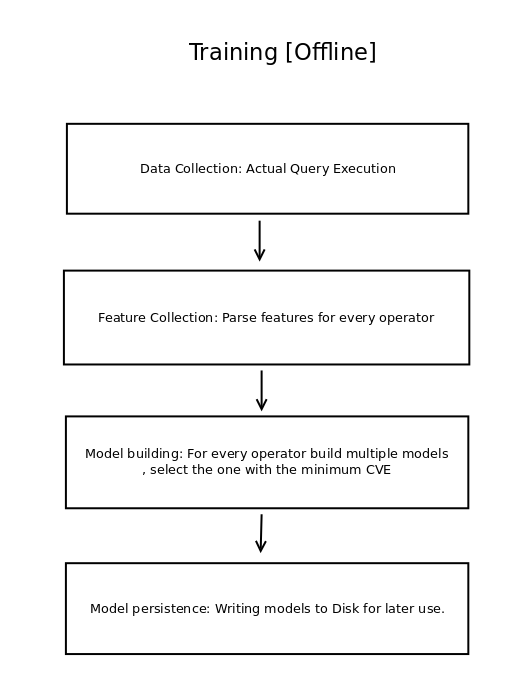
\includegraphics[width=\textwidth]{training.png}
%	  \caption{Operator level approach to Execution time prediction}
%	\end{figure*}
	
	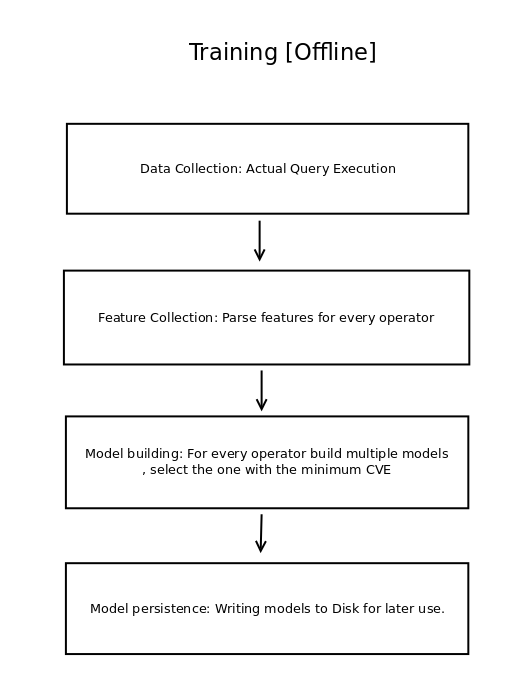
\includegraphics[scale=0.4]{training.png}
	

	In this section, we elaborate on the overview of the approach which consists of 2 phases. Like 
	most other machine learning approaches, the first phase is an off-line training phase and the 
	second is on-line testing phase.
	During the training phase, we construct number of different 
	models for each type of physical database operator(e.g.,  Sort-Merge Join, Nested Loop, Index Nested 		Loop,..). Each operator will be associated with so called 'Best-Fit' model which will be determined 
	based on the Operator model selection described in section 3.1. This model will be invoked for the
	purpose of estimating the execution time for a certain operator. Since there are only finite number of 	operators and only a couple of physical implementations for them, the space consumption is not 				excessive. 

\hfill
	
	During the testing phase, we actually run the query to get the true cardinality estimates. While this
	seems to contradict the whole estimation problem, right now this is required because the focus is on
	solving the modeling problem given the actual cardinalities. The more practical scenario i.e., where
	we we only the know the estimated cardinalities, is a much harder problem as now the models also need 
	to be Robust to the errors in cardinality estimates. This is the natural follow-up work to do. Once 
	after the execution of the query, we need to extract features depending on the operator and invoke 
	the Best Fit model (which is already computed during training phase) to get an estimate. We sum up 
	costs for all the operator present in the plan tree to finally give an estimate of execution time. 	
	
	
TO-DO :  
2. Describe the concept of multiple models for a single operator.
3. How do we select the best one among them. (Mention that current experiments don't use this idea, only one a simple non-linear model is used for all models with 2 features) 


Analytical approaches problems: 

counting the numbers of pages read is not sufficient as the discrepancy between random and sequential I/O is tremendous.

%%%%%%%%%%%%%  This can be followed by several other sections
	\section{Training and Model selection}
	Before we describe the concept of multiple models for an operator, we shall present the motivation 
	for doing so. While the statistical models can find the complex non-linear dependencies between 			features and the target, they cannot model the interaction among operators which might
	affect the target value. 
     
	Consider the classic example of Sorting, where in the target variable (execution time) is 
	proportional to $N_{l}$ log$N_{l}$. Unless this is used as a feature, the accuracy of the resulting 
	model can be disappointing. Since we don't know the right function to be used beforehand, 
	we explore the possible set of functions listed bellow and select the one with the 
	minimum estimation error. We've used functions that are similar to the one's defined in 					\cite{robustIISc}.
	
	\begin{itemize}
	\item Linear: $a_{0} N_{l} + a_{1} N_{r}$ 
	\item Quadratic: $a_{0} N_{l}N_{r}$ , $a_{0} N_{l}N_{l}$ , $a_{0} N_{r}N_{r}$ \ldots
	\item Logarithmic: $a_{0} N_{l} log(N_{r}) , a_{0} N_{r} log(N_{l}) $ .. 
	\item Exponential: $a_{0} N_{l} ^ {N_{r}}$  	
	\end{itemize}	
	
	To illustrate the use of the functions in more details, we have plotted the curves with 
	different possible functions for QuickSort as well as IndexNestedLoop operator. For the purpose
	of generating curves for QuickSort we have used the following Query template 
	
	\begin{framed}
	\begin{verbatim}
	Select * from orders
	where o_orderkey <= :varies 
	order by o_totalprice
	\end{verbatim}
	\end{framed}
	
	%We now show the observations for logarithmic and quadratic functions.
	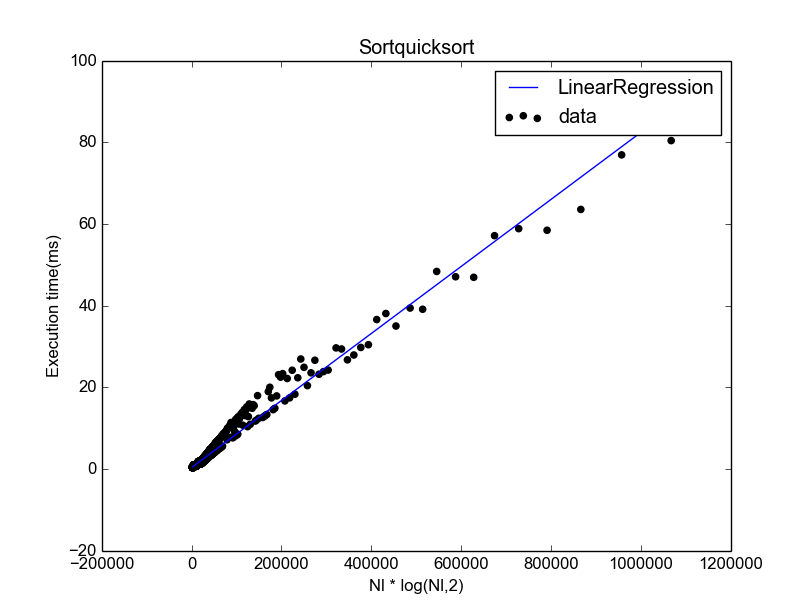
\includegraphics[scale=0.38]{Plots/quicksortnlogn.png}	
	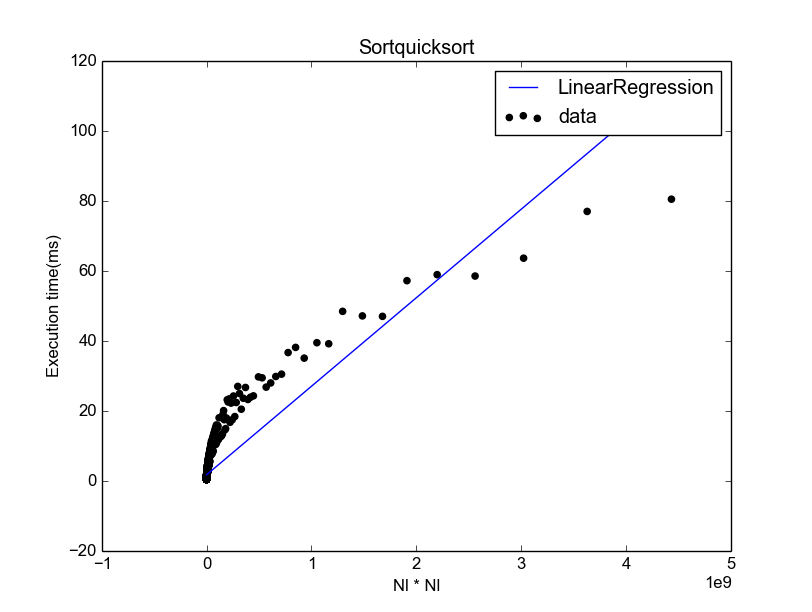
\includegraphics[scale=0.35]{Plots/quicksortnl2.png}	

	Unsurprisingly, logarithmic function fits better than the quadratic. 
	While in some cases (Such as QuickSort) the appropriate function is obvious from SQL
	query processing, it does not hold for all operators. 
	For example, consider Nested Loop Join which 
	can be modeled with quadratic functions in general but when the inner relation has an index 
	the same model produces estimates estimates which are 
	"off" by orders of magnitude. In the following example,
	we take an exploratory approach to determine the best function for the Index Nested Loop operator.
	As in the case of QuickSort we have used the following query template to generate the required
	data.
	
	\begin{framed}
	\begin{verbatim}
	select * from lineitem,orders
	where l_orderkey = o_orderkey 
		  and l_orderkey<= : varies;
	\end{verbatim}
	\end{framed}
	
	
	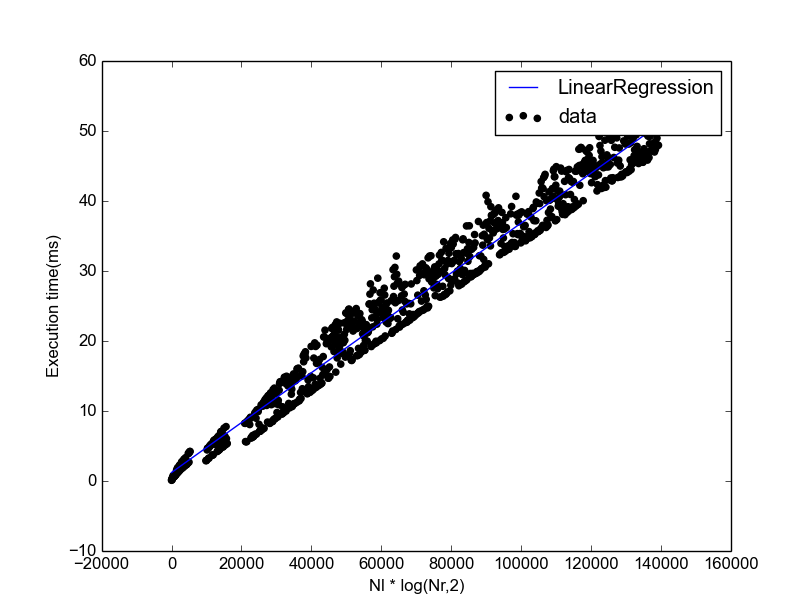
\includegraphics[scale=0.37]{Plots/nil-nlnrlog2.png}	
	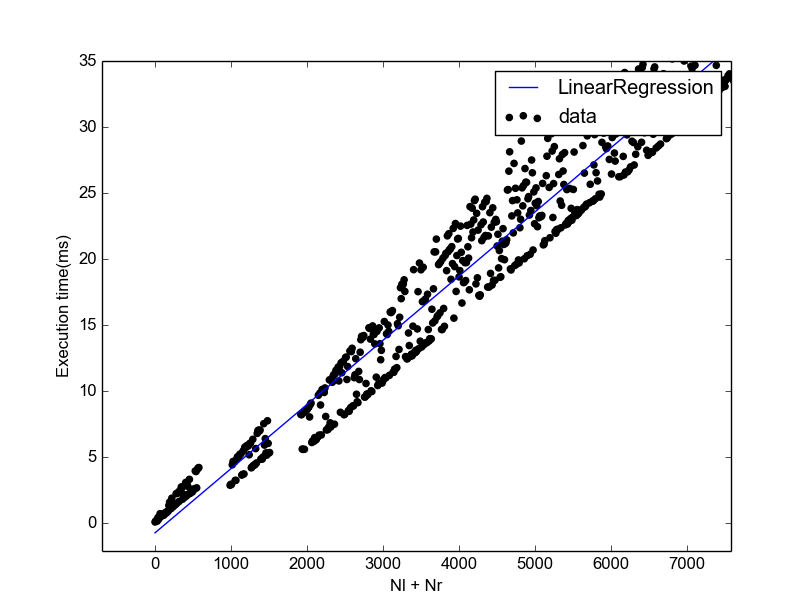
\includegraphics[scale=0.37]{Plots/nil-nl+nr.png}	
	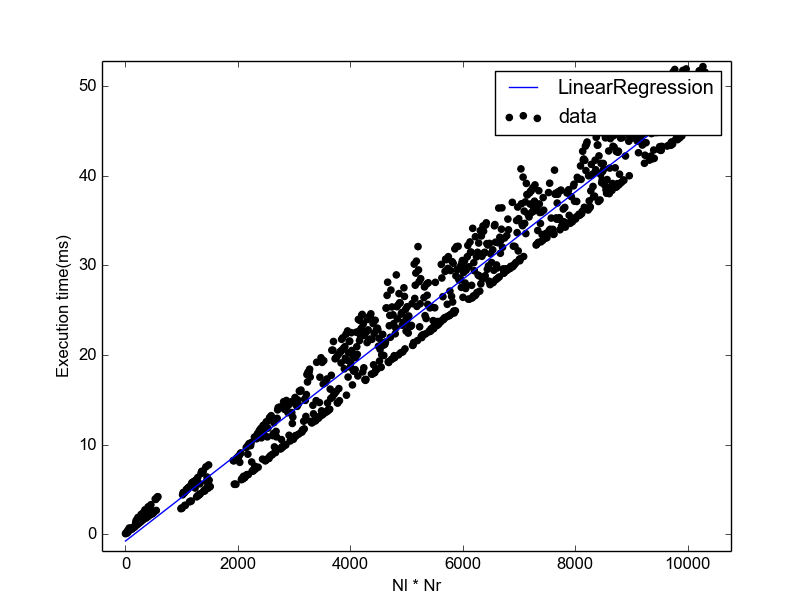
\includegraphics[scale=0.37]{Plots/nil-nlnr.png}	
	
	Out of the above 3 functions, $N_{l} log(N_{r})$ fits data better than other functions. 	
	\subsection{Best Fit Model}	
	Best fit model $M_{O}$ for an Operator $O$ is the model which has the minimum estimation errors 
	for the set of training queries. The estimation error is computed as follows,
	
	\begin{center}
	$\dfrac{1}{n} \sum\limits_{i=1}^n \left| Actual_{i} - Estimated_{i} \right|$
	\end{center}
	
	\section{Preliminary Experiments}
	\subsection{Setup}
	Our experimental study uses TPC-H decision support benchmark \cite{TPCH} on the top of 
	PostgresSQL. The details are as follows, 

	\begin{itemize}
	\item Database Management System : PostgreSQL 9.4
	\item Data sets and workload: We created 1GB TPC-H database
	according to the specification. The primary key indices as indicated
	in the TPC-H specification were created for both databases. We have excluded Query 1,21  
	To keep the training time under control, and Queries 15 as it creates a view which is not yet
	supported in our work. This resulted in 19 out of 22 TPC-H queries being used for training. We've 
	used TPC-H qgen tool to generate 10 instances of each of the 19 queries, resulting in a total of 190 
	queries.
	
	\item Hardware: The queries were executed on a machine
	with 8GB RAM running Ubuntu. buffer pool size was set to 1GB (25\% of the total RAM as the rule
	of thumb). All queries were executed sequentially with cold start
	(i.e., OS buffers flushed before the start of each query).
	
	\item Statistical Models: As of now, we have limited our experiments to at-most 2 features (Input 			cardinalities $N_{l} , N_{r}$). For evaluating the best-fit model we have used linear regression 			models (available from python's sckit-learn \cite{sckit})
	
	TODO : 
	1. Histogram of TPC-H errors.
	2. table with distribution of MRE.
	3. Performance operator wise. Box plot
	4. Insights : which operators are hard to predict
	
	\end{itemize}		
	
	\subsection{Prediction with Optimizer cost models}		
	We start with the results showing that Optimizer's estimates are a poor indication of the real
	execution time. For this purpose, we have taken 19 of 22 queries (To make a fair comparison with 
	our approach we've excluded the 3 templates for the reason stated earlier). The actual execution time
	and prediction times are computed using \textit{Explain Analyze} command of Postgres. The values 			collected are averaged over 5 runs.
	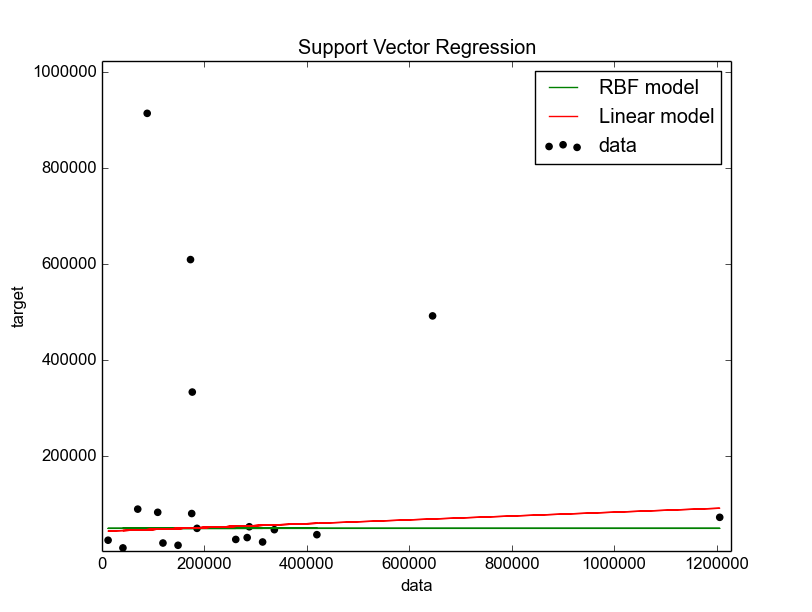
\includegraphics[scale=0.45]{optcost.png}
	
	We've plotted the linear regression line resulting from fitting these points 
	using linear least-squares regression 
	(which can be seen as an error-minimizing mapping of the
	optimizer-estimated cost (which is not measured in ms) to CPU-
	time). As we can see, even for the mapping chosen to minimize
	the overall error, there are significant differences between the estimated CPU cost 
	and real CPU time for many queries. Similar
	observations have been made in other works as well \cite{MSR,ICDE2012}

	Note that while the final estimate made by the optimizer may not be an accurate reflection of
	real execution time, the estimates provided at a finer level (i.e., plan level, operator level etc.) 
	are quite useful. In the next section, we show how we can use optimizer's estimates at operator level 
	and produce an estimate for overall execution time.
		
	\subsection{Operator level modeling}
	PostgreSQL query optimizer provides the wide range of information at multiple levels. For example, 
	for the Hash operator, it provides the following information.
	
	\begin{center}
	\begin{tabular}{ |c|c| } 
	 \hline
		Node Type& Hash \\
		Parent Relationship& Inner\\
		Startup Cost& 4.45\\
		Total Cost& 4.45\\
		Plan Rows& 1\\
		Plan Width& 117\\
		Actual Startup Time& 0.017\\
		Actual Total Time& 0.017\\
		Actual Rows& 6\\
		Actual Loops& 1\\
		Hash Buckets& 1024\\
		Hash Batches& 1\\
		Original Hash Batches& 1\\
		Peak Memory Usage& 1\\
	 \hline
	\end{tabular}
	\end{center}
	
	While all of these attributes may not be candidates for features (i.e may not impact execution time),	some do. We can use the knowledge of SQL Query processing to select relevant features and determine the Best Fit Model as described earlier(Section 4.1). In this set of experiments, we are limiting
	ourselves to the feature 'Actual Rows' (i.e, Input cardinalities). In the case of binary operator nodes (such as
	Nested Loop), we are considering both left and right input cardinalities. Please note that 
	a) the proposed feature set should not be considered complete as it may not capture all the properties that impact execution time, we shall review these set of features from time to time as we make progress in this work.  b) More number of features 	correspond to increased training time and since the computation of Best Fit Model is exponential to the number of features, we should select as few features as possible to make the computations tractable. 
	
	To ensure that the trained model is not over-fitting the data, we have generated training and testing queries do not contain identical instances of same query (i.e, Same query with same selectivities is not allowed). 
	
	\begin{center}
	\begin{tabular}{ |c|c|c|c| } 
	\hline
	  Model & Minimum & Maximum & Mean\\ [0.5ex] 
	 \hline
	 Optimizer & 0.032  & 47.68 & 8.33 \\
	 Our model & 0.003 & 2.61 & 0.53 \\
	 \hline
	\end{tabular}
	\end{center}

	\begin{figure*}[!t]
	  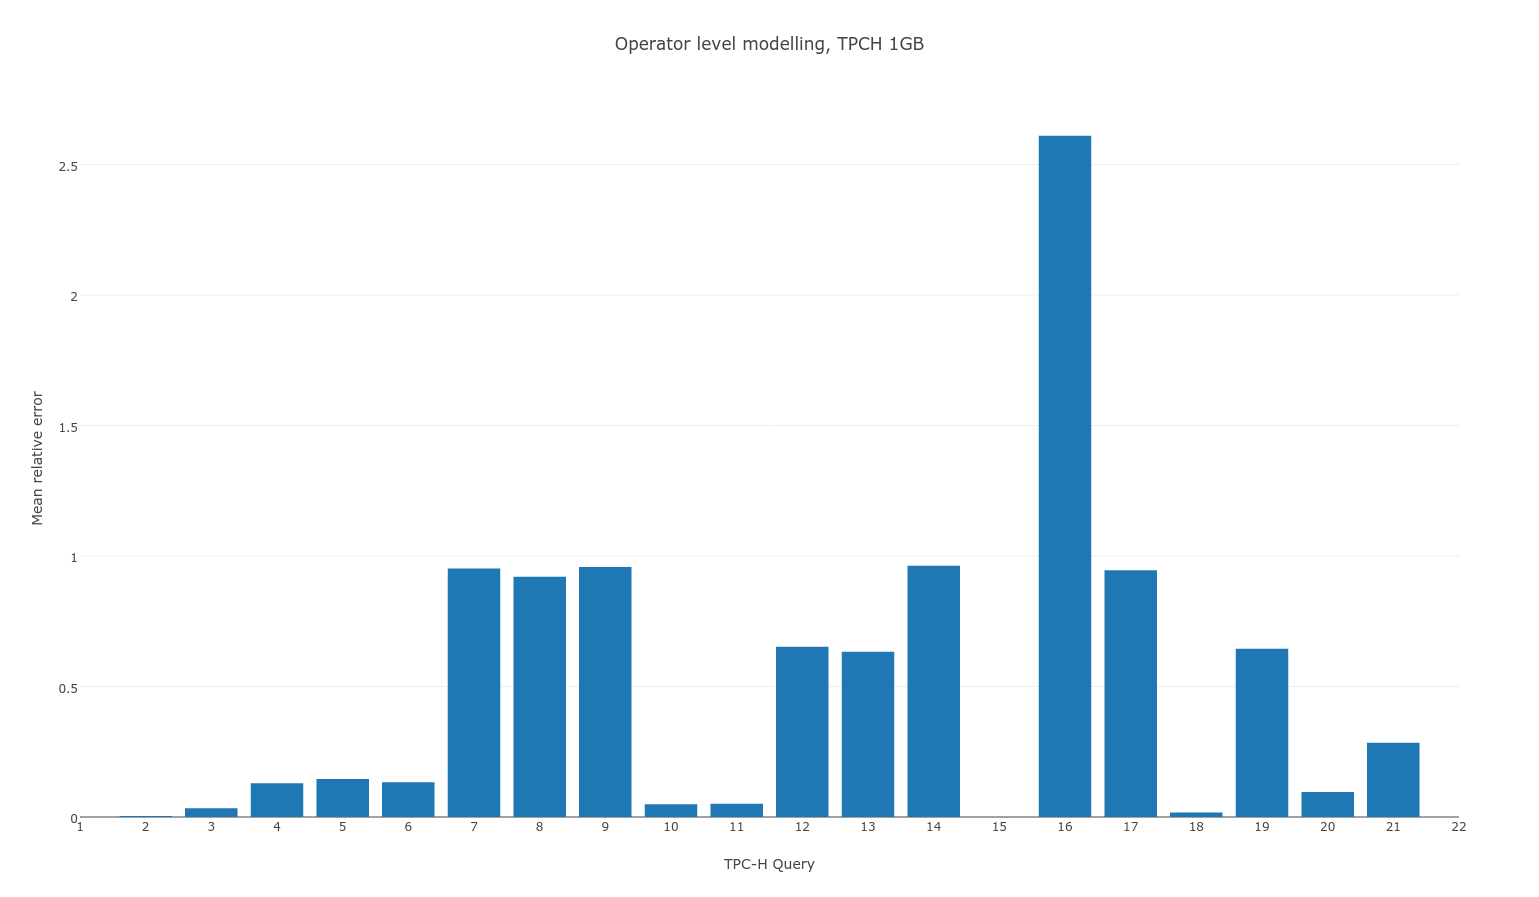
\includegraphics[width=\textwidth]{tpch-1gbres.png}
	  \caption{Operator-level modeling ,Errors by Template (1GB)}
	\end{figure*}

%	Give a background about Static and dynamic workload.  
%	do experiments at 2 stages
%	1. Act vs Act
%	2. Est vs Est(Bias towards estimated cardinalities)
%	For each type of above scenario, do testing for tpc-h queries 
%	(tpc-ds in future)
%	At different scales to see the model's ability to predict.
%	For midterm you should be having result for 1 as well as 10 GB.
%	For each above dataset, 
%	Results should convey L1 (MRE) as well as queries that are within 
%	[0-0.5] [0.5-1] [1-1.5] 

	\section {Related work}
		
	
	\section{Conclusions and Future Work}
	In this work, we have presented learning based approach at a finer granularity than whats proposed earlier in the literature. By learning at operator level we have shown that the model can generalize to the queries which are unseen during the training because of the fundamental property that execution time is upper bounded by execution time of individual operators present in the plan tree. 
	There remains a lot of work to be done. Currently feature set is limited, extending it will definitely improves accuracy and generality. However since the best-fit algorithm is exponential to number of features, it remains as a challenging work.
%	We have assumed that we are getting true cardinalities, where in the practical scenario they will often have magnitude of errors. If we train the model with optimizers estimates instead of true cardinalities, the model to certain extent can have a bias towards estimation errors. On the other hand, we can have partial executions 
	
Also, interaction that happen within query makes accurate execution time prediction hard. For example, pipelining speeds up the query processing and is the primary source of over-estimation. Capturing these in the cost model is a challenging and has got the attention in recent years \cite{concurrent}. As mentioned earlier, we are not currently not addressing prediction in case of concurrent query execution. There is already some promising work in addressing this problem \cite{Ahmed,qshuffler}. It remains as an interesting future work to see how we can extend the features so that we can capture the execution time behavior under concurrent workloads.
	
	\begin{thebibliography}{9}
	\bibitem{ganapathi} 
	A. Ganapathi, H. A. Kuno, U. Dayal, J. L. Wiener, A. Fox, M. I. Jordan,
	and D. A. Patterson. Predicting multiple metrics for queries: Better
	decisions enabled by machine learning. In ICDE, 2009.
	
	\bibitem{MSR}
	Li, Jiexing, et al. "Robust estimation of resource consumption for sql queries using statistical 			techniques." Proceedings of the VLDB Endowment 5.11 (2012): 1555-1566.
	
	\bibitem{ICDE2012}
	Akdere, Mert, et al. "Learning-based query performance modeling and prediction." Data Engineering 			(ICDE), 2012 IEEE 28th International Conference on. IEEE, 2012.	
	
     \bibitem{adaptive} 
     S. Guirguis, M. A. Sharaf, P. K. Chrysanthis, A. Labrinidis, and
	K. Pruhs. Adaptive scheduling of web transactions. In ICDE, 2009.
	
	\bibitem{robustIISc}
	Harish, D., Pooja N. Darera, and Jayant R. Haritsa. "Identifying robust plans through plan diagram 			reduction." Proceedings of the VLDB Endowment 1.1 (2008): 1124-1140.
	
	\bibitem{concurrent}
	Wu, Wentao, et al. "Towards predicting query execution time for concurrent and dynamic database 			workloads." Proceedings of the VLDB Endowment 6.10 (2013): 925-936.
	
	\bibitem{Ahmed}
	Ahmad, Mumtaz, et al. "Modeling and exploiting query interactions in database systems." Proceedings of the 17th ACM conference on Information and knowledge management. ACM, 2008.
	
	\bibitem{qshuffler}
	Ahmad, Mumtaz, et al. "Qshuffler: Getting the query mix right." Data Engineering, 2008. ICDE 2008. IEEE 24th International Conference on. IEEE, 2008.

	
	\bibitem{forecasting}
	Makridakis, Spyros, Steven C. Wheelwright, and Rob J. Hyndman. Forecasting methods and applications. John Wiley, 2008.
	
	\bibitem{TPCH}
	TPC-H benchmark specification, http://www.tpc.org/tpch/
	
	\bibitem{TPCDS}
	R. Othayoth and M. Poess, The making of tpc-ds, in VLDB
	06: Proceedings of the 32nd international conference on Very
	large data bases. VLDB Endowment, 2006, pp. 1049Ð1058
	
	\bibitem{sckit}
	Scikit-learn: Machine Learning in Python, Pedregosa et al., JMLR 12, pp. 2825-2830, 2011.
	
	\bibitem{opthet} 
	Du, Weimin, Ravi Krishnamurthy, and Ming-Chien Shan. "Query optimization in a heterogeneous dbms." 		VLDB. Vol. 92. 1992.
	\bibitem{activeSLA}
	Xiong, Pengcheng, et al. "ActiveSLA: a profit-oriented admission control framework for database-as-a-		service providers." Proceedings of the 2nd ACM Symposium on Cloud Computing. ACM, 2011.	
	\bibitem{progress}
	Mishra, Chaitanya, and Nick Koudas. "The design of a query monitoring system." ACM Transactions on 		Database Systems (TODS) 34.1 (2009): 1.
	
	\end{thebibliography}
	\end{multicols}
\end{document}
